\chapter{Calibración de probabilidades}\label{cap:calibracion}

\section{Diagnóstico inicial}

Para cada modelo entrenado se computan las probabilidades $\hat{p}_k(x)$
sobre la partición de prueba y se evalúan:
\begin{itemize}[leftmargin=*,itemsep=0.2em]
  \item \emph{Expected Calibration Error} (ECE) con $M = 15$ bins
        equidistantes.
  \item Diagrama de fiabilidad: gráfico
        $\bigl(\mathrm{conf}(B_m),\,\mathrm{acc}(B_m)\bigr)$ junto a la
        diagonal.
  \item Histograma de confianzas $\max_k \hat{p}_k(x)$.
\end{itemize}

\section{Métodos \emph{post-hoc} considerados}

Los siguientes métodos se incluyen como referencia metodológica y como
línea de extensión. En el experimento final no se ajustan calibradores
\emph{post-hoc}; se reporta únicamente el diagnóstico de las
probabilidades originales.

\subsection{\emph{Temperature scaling}}

La temperatura $T > 0$ reescala los \emph{logits} previos a
\emph{softmax}:
\[
  \hat{p}^T_k(x) = \softmax_k\bigl(z(x) / T\bigr).
\]
$T$ se estimaría por NLL sobre un conjunto de calibración
estratificado, resolviendo el problema convexo
unidimensional
\[
  \hat{T} = \argmin_{T > 0}\;
  -\sum_i \log \softmax_{y_i}\bigl(z(x_i) / T\bigr).
\]
Este método preserva el ranking de las predicciones y, por tanto, la
exactitud, modificando exclusivamente las probabilidades.

\subsection{Regresión isotónica}

Aplicada \emph{one-vs-rest}, ajusta para cada clase $k$ una función no
decreciente $g_k : [0, 1] \to [0, 1]$ minimizando
$\sum_i (g_k(\hat{p}_k(x_i)) - \mathbb{1}\{y_i = k\})^2$ sujeta a
monotonía, mediante el algoritmo \emph{Pool Adjacent Violators}. Tras el
ajuste se renormalizan las probabilidades para que sumen 1.

\section{Evaluación}

Sobre la partición de prueba se reporta el diagnóstico sin recalibración
\emph{post-hoc}:
\begin{itemize}[leftmargin=*,itemsep=0.2em]
  \item NLL.
  \item ECE.
  \item \emph{Brier score} multiclase.
  \item Diagrama de fiabilidad del modelo neuronal.
\end{itemize}

\begin{table}[h]
  \centering
  \begin{tabular}{llccc}
    \toprule
    Modelo & Calibración & NLL & ECE & Brier \\
    \midrule
    TF-IDF + LR       & ninguna & 1.0897 & 0.1585 & 0.6342 \\
    DeBERTa-v3-small  & ninguna & 0.8070 & 0.1277 & 0.4231 \\
    \bottomrule
  \end{tabular}
  \caption{Diagnóstico de calibración sin recalibración \emph{post-hoc}.}
  \label{tab:calibration}
\end{table}

\begin{figure}[h]
  \centering
  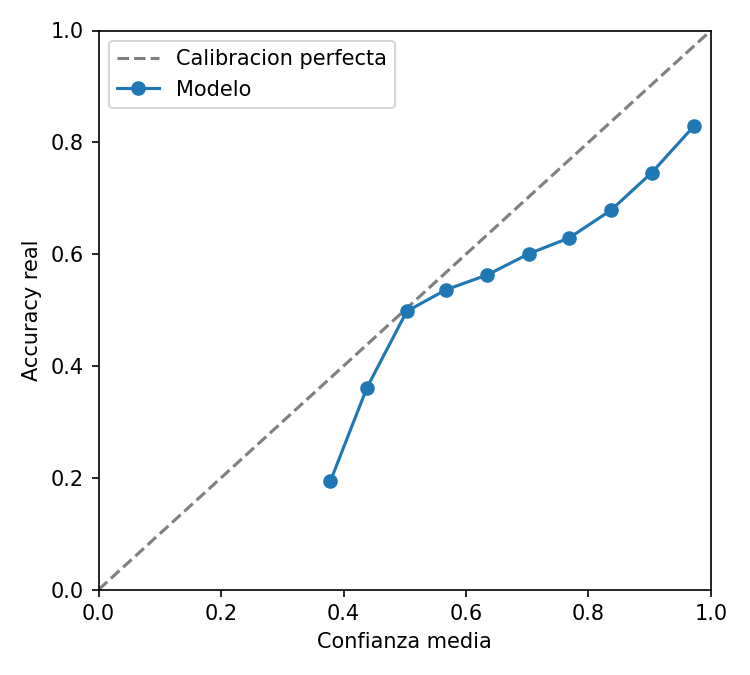
\includegraphics[width=0.78\textwidth]{../../research-stats/reports/figures/deberta_v1_reliability.png}
  \caption{Diagrama de fiabilidad de DeBERTa-v3-small sobre la partición de prueba.}
  \label{fig:deberta-reliability}
\end{figure}

El valor ECE de DeBERTa-v3-small (0.1277) mejora al baseline, pero no
es lo bastante bajo como para considerar las probabilidades finales
plenamente calibradas. Por ello la calibración por temperatura o
isotónica se mantiene como extensión natural antes de usar los scores
como probabilidades operativas en decisiones de alto impacto.

\section{Implicaciones para la regla de agregación}

La calibración es prerequisito para la regla de agregación del
capítulo~\ref{cap:agregacion}: dicha regla asume que
$\hat{p}_k(c, e_i)$ aproxima $\Prb(Y = k \mid c, e_i)$. Sin
calibración adecuada, los umbrales de decisión y los valores
agregados pierden interpretación probabilística.
